\chapter{Background}

\section{Conceptual modeling of software systems}

Conceptual modeling is an integral part of system construction. A conceptual model can be defined as a skeleton of the system. In the context of information systems this term is often used interchangeably with the term "conceptual schema", which comes from the world of relational database management systems (RDBMS). Conceptual schema describes the structure of the database from a high-level perspective. More specifically, it identifies the core concepts and relationships between them. It does not, however, include any internal details about the database.

For example, in a banking system domain, the conceptual schema might define concepts such as \textit{banking accounts and transactions}, as well as their relationship. One common language for expressing conceptual schemas is UML. Consider the banking example illustrated as a UML class diagram:

\n

\begin{figure}[H]\centering
    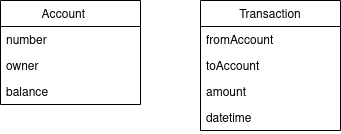
\includegraphics[scale=0.65]{images/banking.drawio.png}
    \caption{UML class diagram for a simplified banking domain}\label{fig:bank}
\end{figure}

Here the conceptual schema consists of two domain entities, or in other words, two identifiable concepts. Both of them are characterized by specific attributes that describe their structure. And what often happens in domain modeling is that the underlying structure of an entity undergoes some kind of modification. For example, consider the diagram below that introduces a new attribute to the \texttt{Account} concept, namely, its creation date:

\begin{figure}[H]\centering
    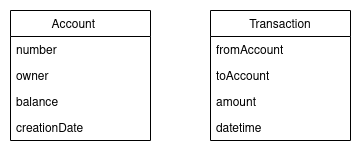
\includegraphics[scale=0.65]{images/banking1.drawio.png}
    \caption{UML class diagram illustrating an additive change of the conceptual model}\label{fig:bank1}
\end{figure}

\n

Modifications on a conceptual level, such as these, must be performed with caution, since they are fundamental in their nature. This means that every part of the system that interacts with a modified concept should be taken into account during verification. However, a simple additive change might not be convincing enough. Here is another example showing an existing attribute being modified:

\begin{figure}[H]\centering
    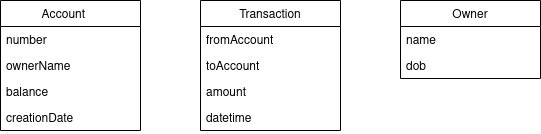
\includegraphics[scale=0.65]{images/banking2.drawio.png}
    \caption{UML class diagram illustrating a breaking change of the conceptual model}\label{fig:bank2}
\end{figure}

The \texttt{owner} attribute of \texttt{Account} has been replaced by \texttt{ownerName}. The \texttt{Owner} concept has also been included in the diagram to illustrate possible consequences of this modification. Given that prior to this change the \texttt{owner} attribute was referring to the \texttt{Owner} concept, some part of a system could be making use of this fact to construct a database query that searches for account owners by their date of birth. Ideally, after the modification has taken place, the system would undergo validation and any incorrectly constructed database queries would be reported. In our example one would expect the validation mechanism to report that the \texttt{Account} concept does not define an attribute \texttt{owner} of type \texttt{Owner}, requiring that part of the system to be modified accordingly to conform to latest changes.

\n

However, the world of software systems is not perfect. Database querying mechanisms work under the assumption that their input is consistent with the actual conceptual schema. If incorrect input is supplied, it will most likely cause the system to fail when it is already running or being tested.

\section{Domain-driven design and its lingo}

Domain-driven design is an approach to conceptual modeling of a specific business domain. Its main aim is construction of a domain model, which translates to a conceptual model of the domain. The fundamental assumption is that a domain consists of entities, that is, concepts, and the relationships between those entities. The term \textit{entity} is used interchangeably with the term \textit{concept}. Every entity is characterized by its \textit{properties} in the same way that every concept is characterized by its \textit{attributes}.

\section{Java programming language}
Java is a compiled, high-level, class-based, object-oriented programming language. In practice it is often used to implement domain-driven software solutions. Domain entities are represented as Java classes, preferably as plain old Java objects (POJOs). Class fields serve as a representation of entity properties.

\n

In contrast with other compiled languages, such as C, Java is characterized by its sophisticated run-time mechanism that provides dynamic capabilities, such as reflection and code modification. Reflection, in particular, makes metaprogramming possible, which allows the program to use other programs, itself included, as data. For example, using reflection it is possible to obtain the type of a class field by its name:

\begin{minted}{java}
class Person {
    private Animal pet;
}

Person.class.getDeclaredField("pet").getType()); // class Animal
\end{minted}

Although this is a powerful programming technique that allows run-time type introspection to take place, it can’t be used to treat the source code of a program as data. The run-time nature of reflection means that it operates on objects constructed from compiled code, that is, the result of translation of source code into another form (bytecode). What this means is that metadata obtained by using reflection exists only at run-time of the program, therefore it is of no use at compile time.

\section{Java annotations}

The Java Language Specification defines a special construct – annotations – that provides data about a program that is not part of the program itself, that is, has no direct effect on the operation of code that is annotated. Annotations may be used to provide additional information to the compiler or to be examined during run-time of the program. We focus on compile time processing of annotations. As an example, the \texttt{@Deprecated} annotation can be used to tell the compiler to generate warnings in places where the annotated element is used.

\begin{minted}[escapeinside=||]{java}
class Transformer {
    @Deprecated
    public static boolean isTransformable(Item item) {
        ...
    }
}

// warn: the method Transformer.isTransformable(Item) is deprecated
Transformer.|\st{isTransformale}|(someItem);
\end{minted}

The annotated method can still be used as if there was no annotation, but the warning makes it clear that the method is no longer supported and its usage is discouraged.

\section{Annotation processing}

Annotation processing, as its name implies, is a mechanism for processing annotations in the source code at compile time. An important distinction from the previously mentioned concept of reflection is that the input of an annotation processor is an AST\footnote{Abstract syntax tree is a tree-like data structure used by the compiler to represent the structure of program source code.} constructed from the source code.

\n

The \texttt{@Deprecated} annotation in the example above is one of the Java built-in annotations. It gets processed by a built-in annotation processor that is a part of the Java compiler.

\n

The standard library of Java includes a common interface to all annotation processors, so programmers can provide their own implementations and tell the compiler to use them. Apart from issuing compile time warnings and errors, annotation processing provides a way of generating code.

\begin{figure}[H]\centering
    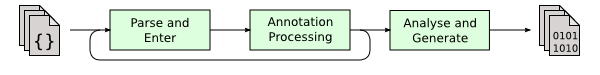
\includegraphics[scale=0.8]{images/javac-flow.png}
    \caption[Compilation process of javac]{Compilation process of \texttt{javac}\footnotemark }\label{fig:javac-flow}
\end{figure}
\footnotetext{Java compiler included in the JDK from Oracle}

Java compilation process can be broken down into three steps:

\begin{enumerate}
    \item The input source files are parsed to build a syntax tree.
    \item All appropriate annotation processors are run until no new files are generated.
    \item The syntax tree is analyzed to generate byte-code.
\end{enumerate}

It is important to mention that step number one may differ across compiler implementations. The main difference lies in the input of a compiler. There is a notion of incremental compilation, which provides an ability to limit the number of source files that are passed as input to the compiler. As opposed to traditional compilation that requires the whole set of source files to be recompiled, an incremental compiler’s input is limited to that portion of the program that was modified.

\n

The built-in annotation processing API in Java has a rich collection of types that model the source language itself, equipping programmers with a powerful abstraction to analyze the syntax tree.\footnote{\texttt{javax.annotation.processing}}
